\documentclass[12pt,a4paper]{article}
\usepackage[UTF8]{ctex}     %先引入ctex
\usepackage[utf8]{inputenc} %再引入inputenc
\usepackage{graphicx}
% \usepackage{lazylatex}
% \tcbuselibrary{documentation}
\usepackage{multicol}
\usepackage{tikz}
\usetikzlibrary{matrix}
\usepackage{pgfplots}
\pgfplotsset{compat=1.17}
\usepackage{xcolor}
\usepackage{listings}
\usepackage{amsmath}
\usepackage{bookmark}
\usepackage{enumerate}
\usepackage{geometry}
\graphicspath{{img/}}
% 边距
\geometry{left=2.0cm,right=2.0cm,top=2.0cm,bottom=3.0cm}
% 大题
\newenvironment{problems}{\begin{list}{}{\renewcommand{\makelabel}[1]{\textbf{##1}.\hfil}}}{\end{list}}
% 小题
\newenvironment{steps}{\begin{list}{}{\renewcommand{\makelabel}[1]{(##1)\hfil}}}{\end{list}}
% 答
\providecommand{\ans}{\textbf{答}:~}
% 解
\providecommand{\sol}{\textbf{解}.~}

% \setminted{breaklines,autogobble,frame=lines,framesep=2mm,fontsize=\scriptsize}

% listings
\definecolor{grey}{rgb}{0.8,0.8,0.8}
\definecolor{darkgreen}{rgb}{0,0.3,0}
\definecolor{darkblue}{rgb}{0,0,0.3}
\lstset{%
    % numbers=left, %行号
    % numberstyle=\tiny\color{grey},
    showstringspaces=false,
    showspaces=false,%
    tabsize=4,%
    frame=shadowbox,%
    basicstyle={\ttfamily\scriptsize},%
    keywordstyle=\color{blue!80!black}\bfseries,%
    identifierstyle=,%
    commentstyle=\color{green!50!blue}\itshape,%
    stringstyle=\color{green!50!black},%
    rulesepcolor=\color{gray!20!white},
    breaklines,
    columns=flexible,
    extendedchars=false,
    %mathescape=true,
    language=c,
}

\begin{document}
\title{\normalsize \underline{计算机系统结构(A)}\\\LARGE 实验 4}
\author{李子龙 518070910095}
\date{\today}
\maketitle

\begin{problems}
    \item[一] \textbf{Cache 可视化工具}
    
    \begin{steps}
        \item[1] 场景一
        
        \begin{itemize}
            \item Cache 命中率为 0\% 。
            
            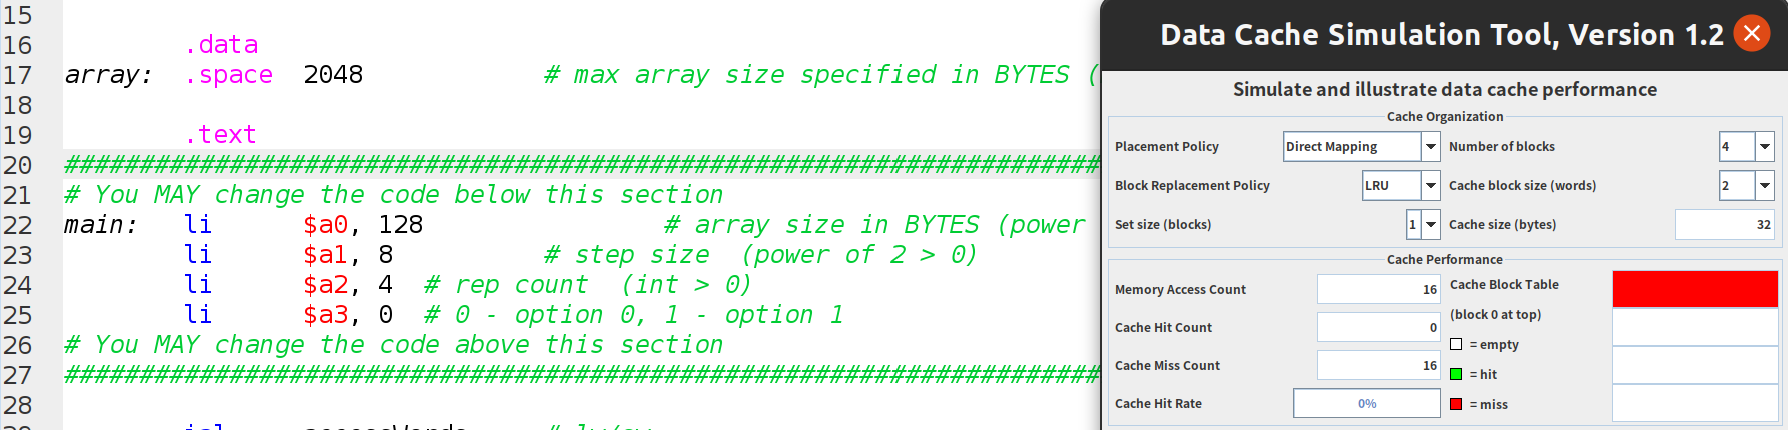
\includegraphics[width=0.7\textwidth]{cache1.png}
            \item \verb"stepsize" 被设定为 8,按照 \verb"int"(4 Bytes) 存储,写入(\verb"option"为0)需要跳跃 32 bytes,只有一组,而一组正好是
            \begin{equation*}
                4\text{ blocks}\times 2\text{ words}\times 4\text{ bytes} = 32 \text{ bytes}
            \end{equation*}
            将会导致每一次的写入都会失效。
            \item 增加 \verb"repcount" 也无法提高命中率,因为上文所述的间隔无法被改变,会一直失效。
            \item 将 \verb"stepsize" 更改为 1,可以将命中率提高至 50\% 。
            
            每对访问第一个失效,第二个命中,在块大小为 2 个字的情形下。

            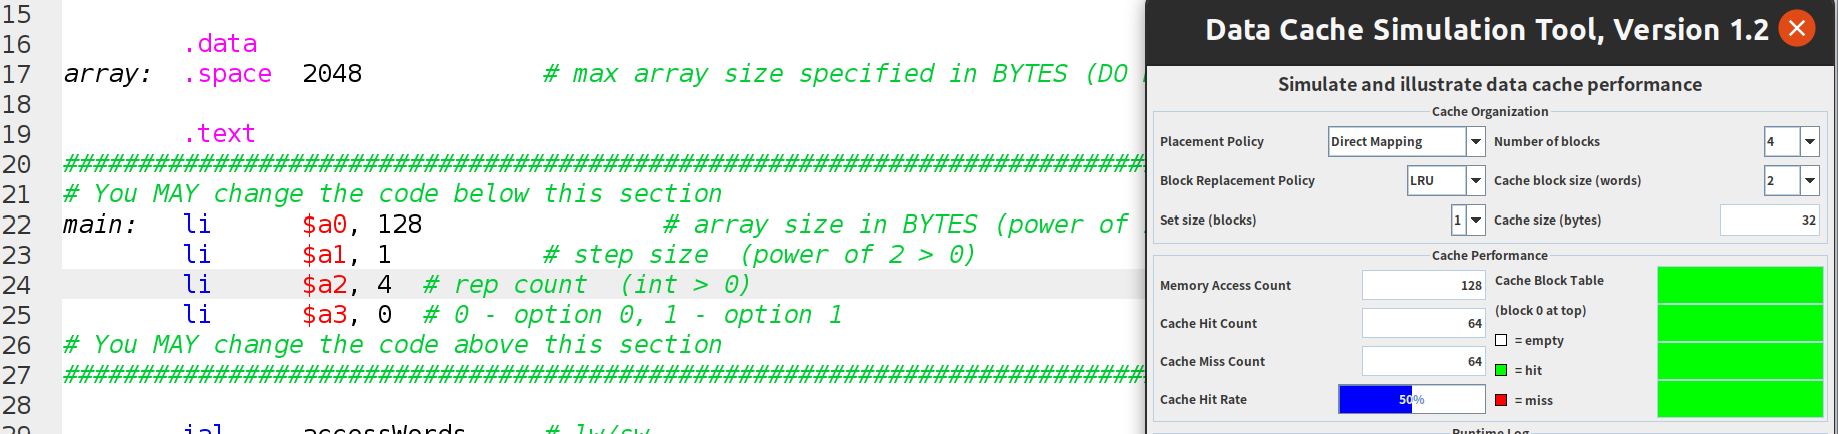
\includegraphics[width=0.7\textwidth]{cache1o.png}
        \end{itemize}

        \item[2] 场景二
        \begin{itemize}
            \item 命中率为 75 \% 。
            
            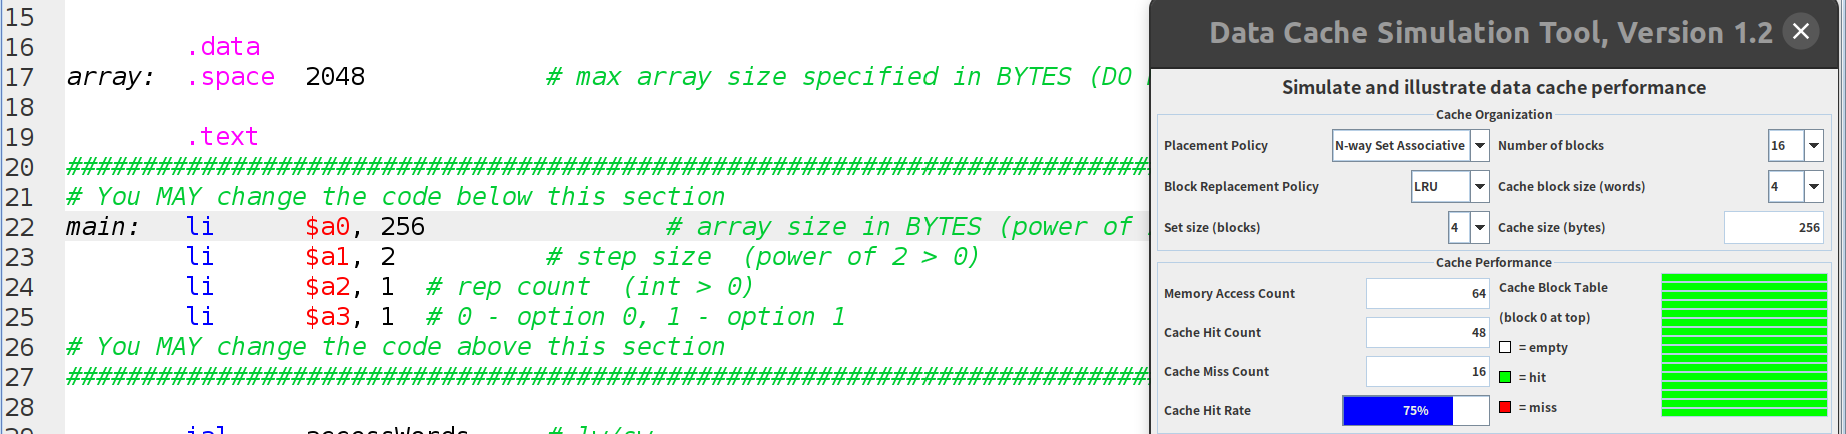
\includegraphics[width=0.7\textwidth]{cache2.png}
            \item \verb"stepsize" 是 2,一块 4 个字,那么相邻的两次读+写,除了第一个读失效,其余均为命中,命中率为 75\% 。
            \item 命中率会接近于 100\% 。因为以第一重复后,所有的数据都进入了 Cache,Cache 大小和数组大小相同:256 bytes,那么后面都不会失效。
            
            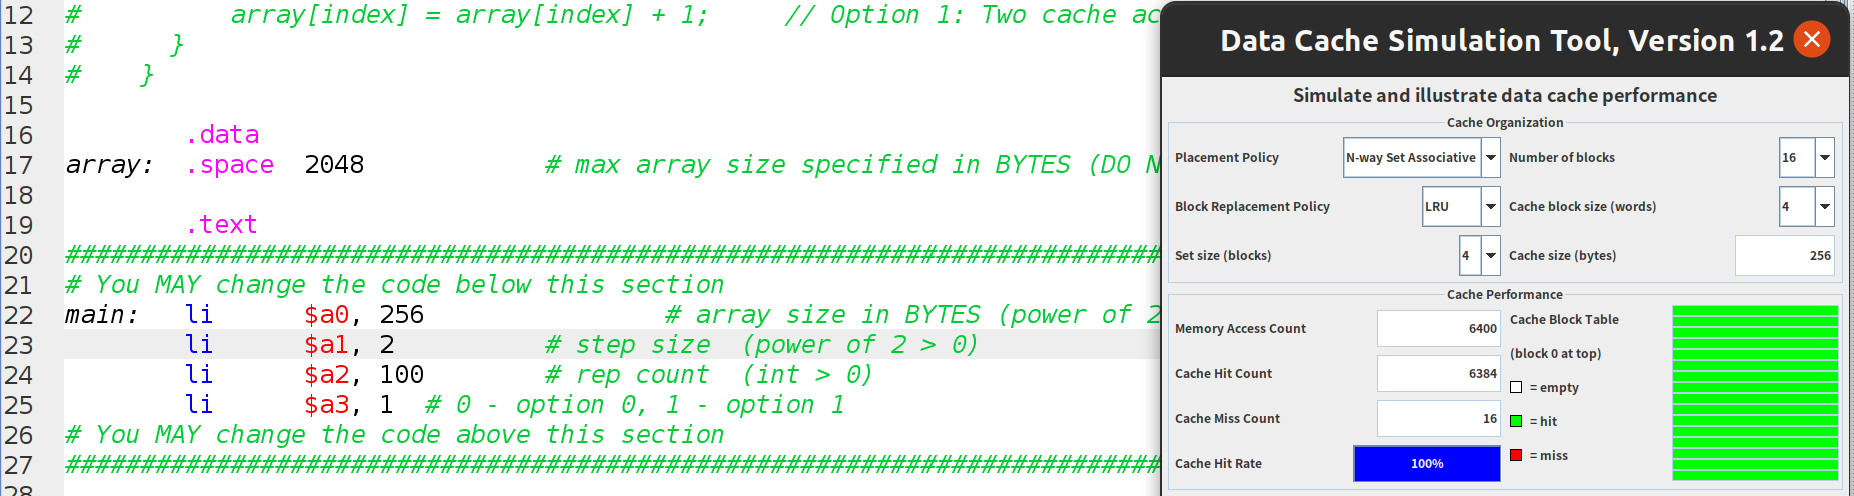
\includegraphics[width=0.7\textwidth]{cache2o.png}
        \end{itemize}
    \end{steps}
    
    \item[二] \textbf{矩阵乘法}
    \begin{itemize}
        \item ikj 性能最好,jki 性能最差。
        
        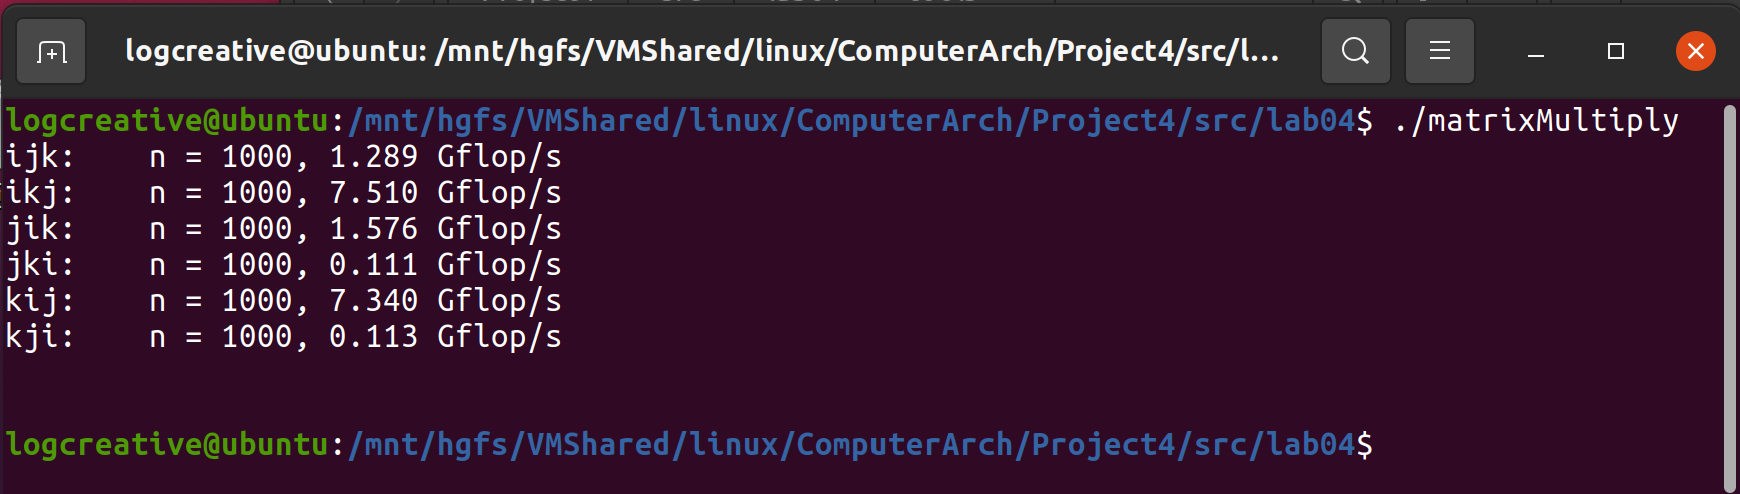
\includegraphics[width=0.8\textwidth]{matrix1.png}

        \item 一致。
        
        \begin{tabular}{c|ccc}
             & 未命中总次数 & 速率1 & 速率2 \\
            \hline
            AB & 1.25 & ijk 1.289 & jik 1.576 \\
            AC & 2.00 & jki 0.111 & kji 0.113 \\
            BC & 0.50 & kij 7.340 & ikj 7.510 \\
        \end{tabular}

        % 影响性能
        不同的算法步长会导致不同的Cache 命中率,从而影响访问时间,也就影响了性能。

        \item 性能得到了改善,除去 kij。
        
        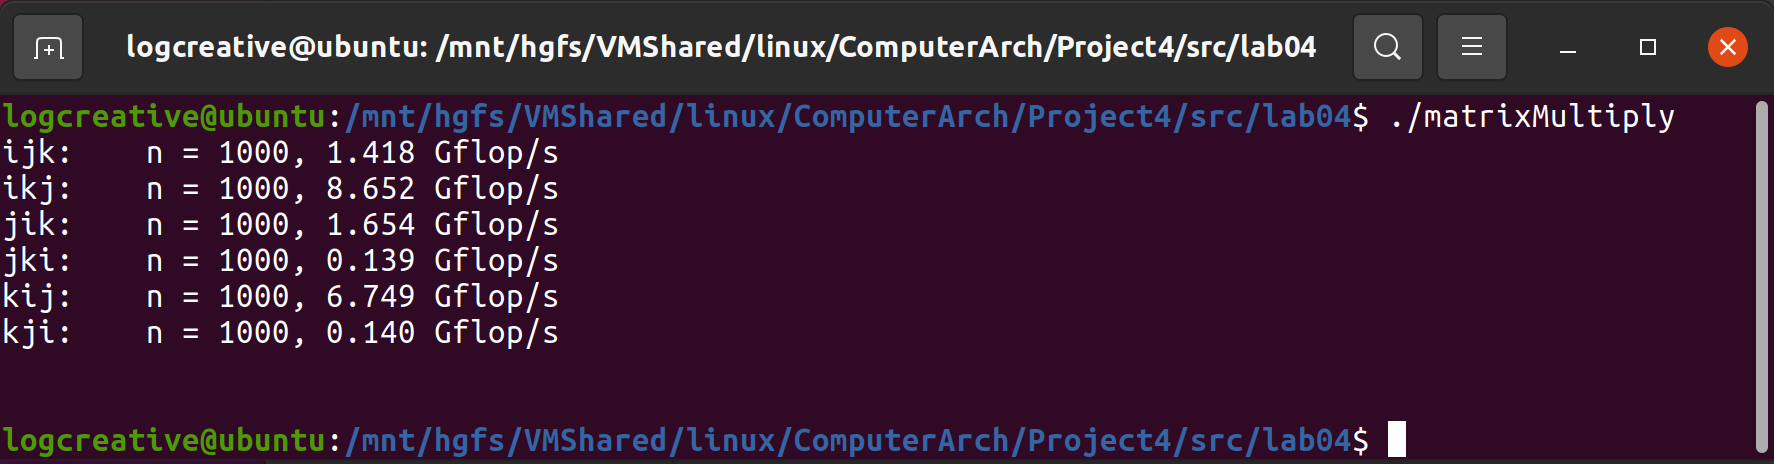
\includegraphics[width=0.8\textwidth]{matrix2.png}

        使用局部变量进行局部加和可以显著减少 Cache 失效率。在有Cache 失效率的情形下,使用局部变量提前预取可以提升性能。

        \item 硬件预取可以大幅降低最低两种算法的失效率,接近于0,而对于另外一些算法效果不明显。
    \end{itemize}

    \item[3] \textbf{矩阵转置}
    
    \verb"transpose_blocking()" 函数的实现如下:
    \begin{lstlisting}
/* Implement cache blocking below. You should NOT assume that n is a
* multiple of the block size. */
void transpose_blocking(int n, int blocksize, int *dst, int *src) {
    // YOUR CODE HERE
    for(int i = 0; i < n; i += blocksize)
        for(int j = 0; j < n ; j += blocksize)
            // (j,i) is the starting element
            // of the block
            for(int x = 0; x < blocksize &&  i + x < n; ++x)
                for(int y = 0; y < blocksize &&  j + y < n; ++y)
                    // (j+y,i+x) is the transposing element
                    // of the matrix.
                    // (i+x,j+y) is the final position.
                    dst[j+y + (i+x)*n] = src[i+x + (j+y)*n];
}
    \end{lstlisting}

    \begin{steps}
        \item[Part 1] 测评结果如下:
        
        \begin{figure}[h]
                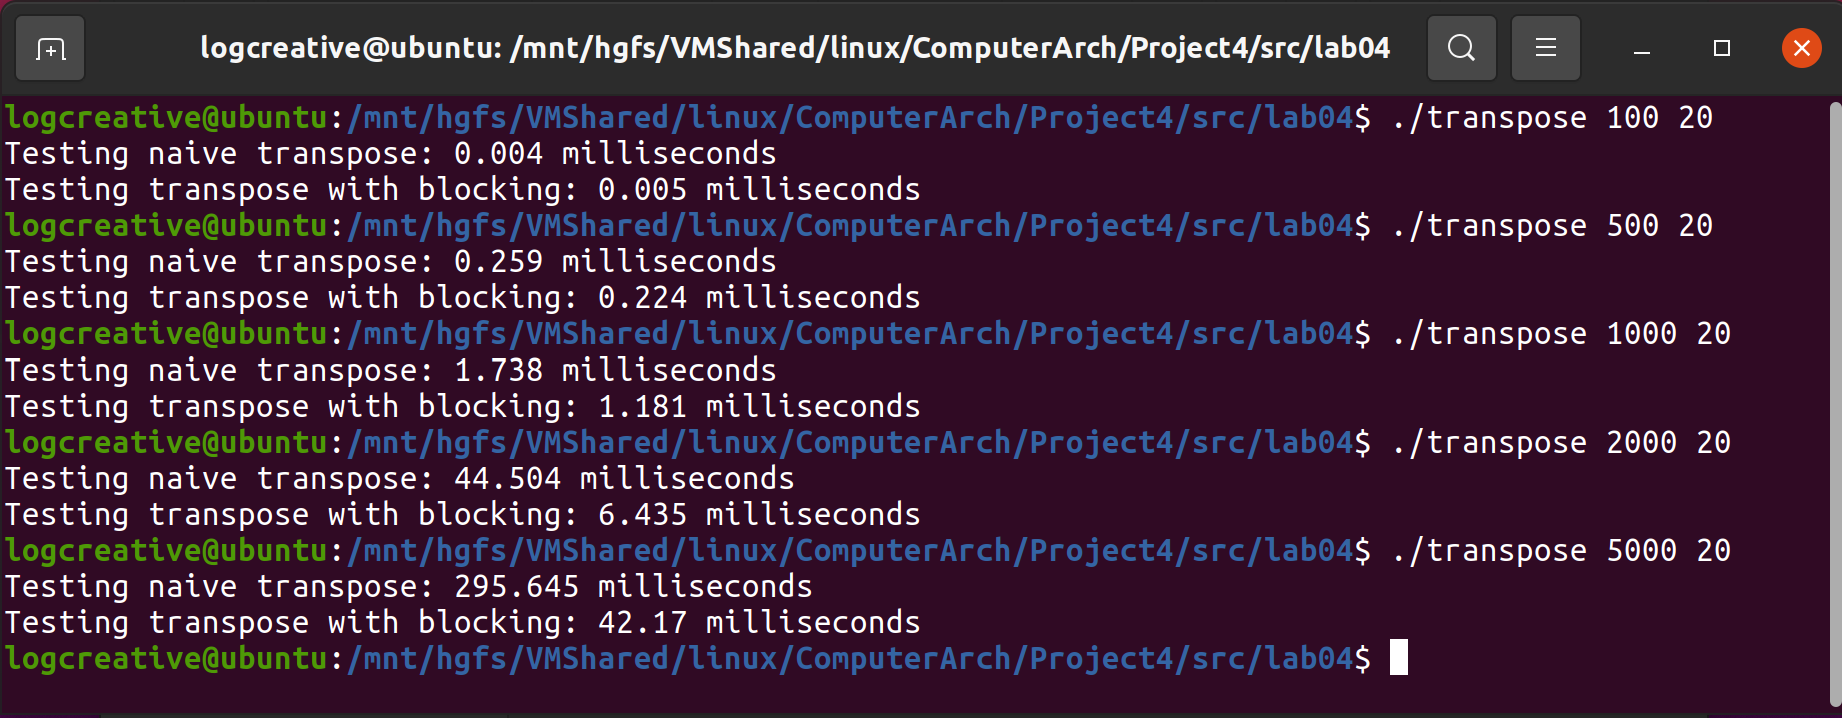
\includegraphics[height=3cm]{transposePart1.png}
                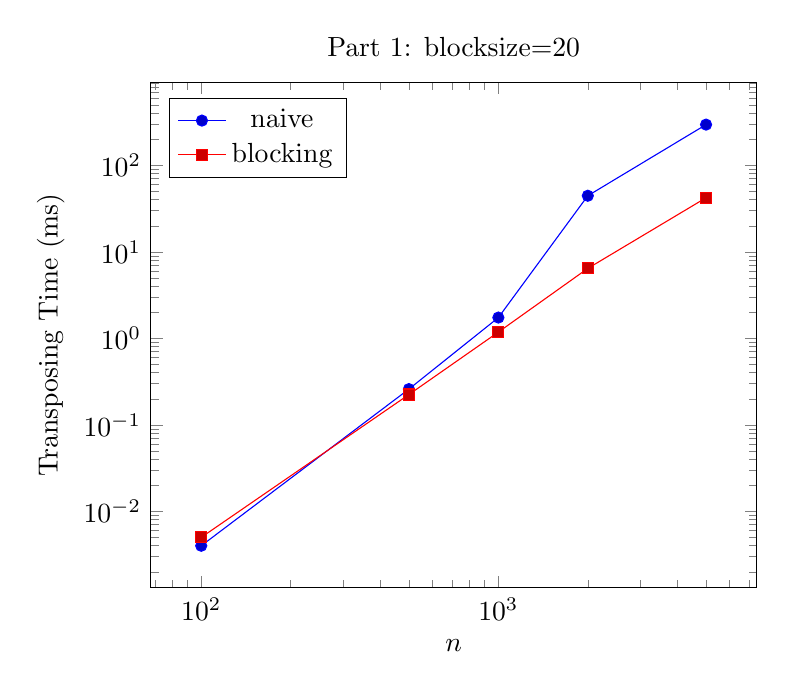
\begin{tikzpicture}
                    \begin{loglogaxis}[legend pos={north west},
                    title={Part 1: blocksize=20},
                    xlabel={$n$},
                    ylabel={Transposing Time (ms)},
                    height=8cm
                    ]
                     \addplot+ [] coordinates { (100,0.004) (500,0.259) (1000,1.738) (2000,44.504) (5000,295.645)};
                     \addplot+ [] coordinates { (100,0.005) (500,0.224) (1000,1.181) (2000,6.435) (5000,42.17)};
                     \legend{naive,blocking,}
                    \end{loglogaxis}
                \end{tikzpicture}
        \end{figure}

        只有当 $n$ 达到 1000 以上时,分块才会比普通方法块,而且规模越大越明显。小型矩阵会因为分块与总规模接近而近似不分块,普通算法和分块算法都不一定能占满 Cache,而且多层循环会增加开销。

        \item[Part 2] 测评结果如下:
        
        \begin{figure}[h]
            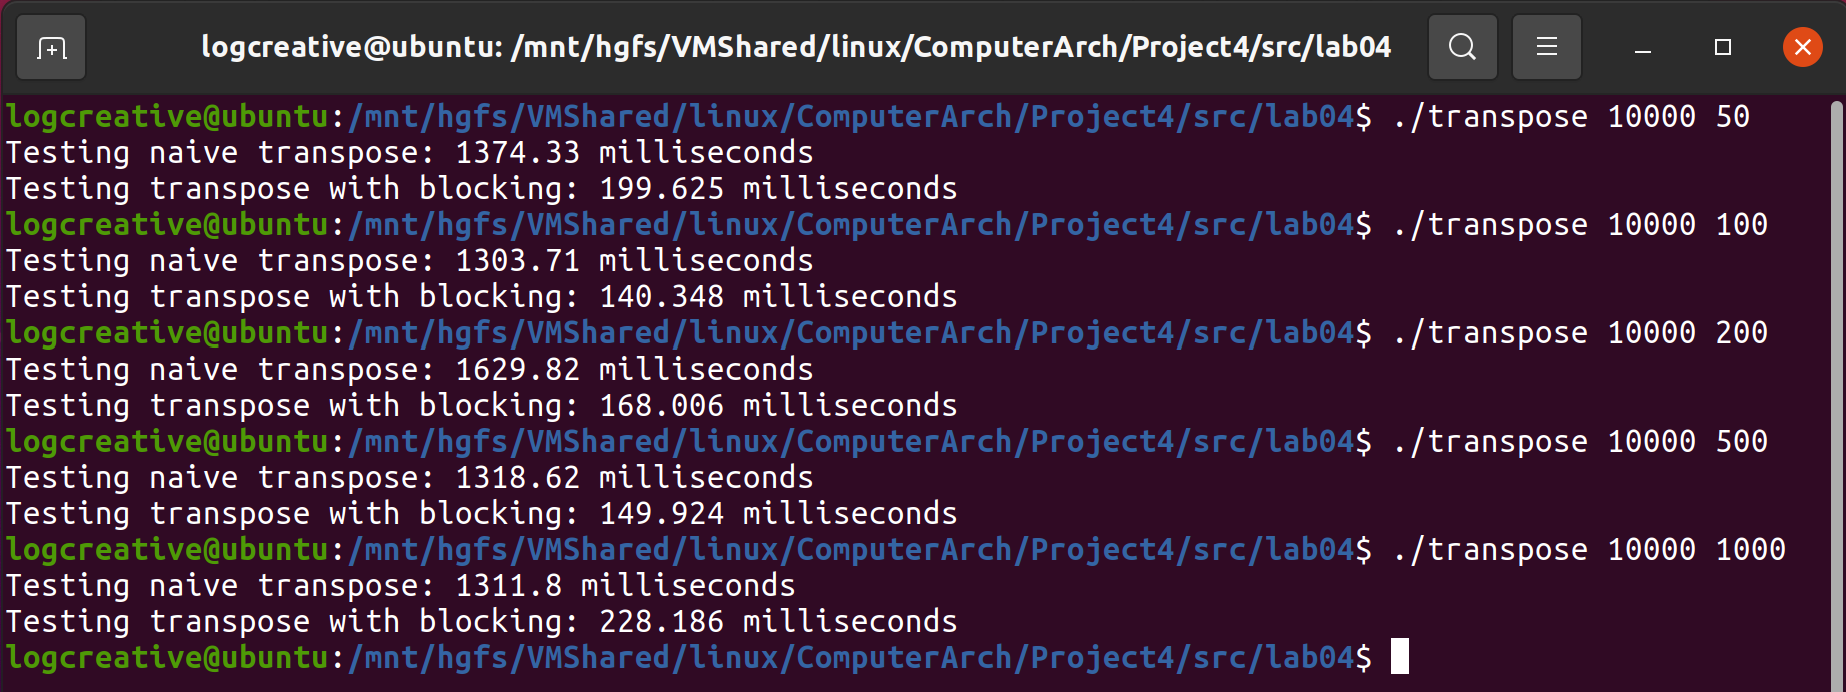
\includegraphics[height=3cm]{transposePart2.png}
            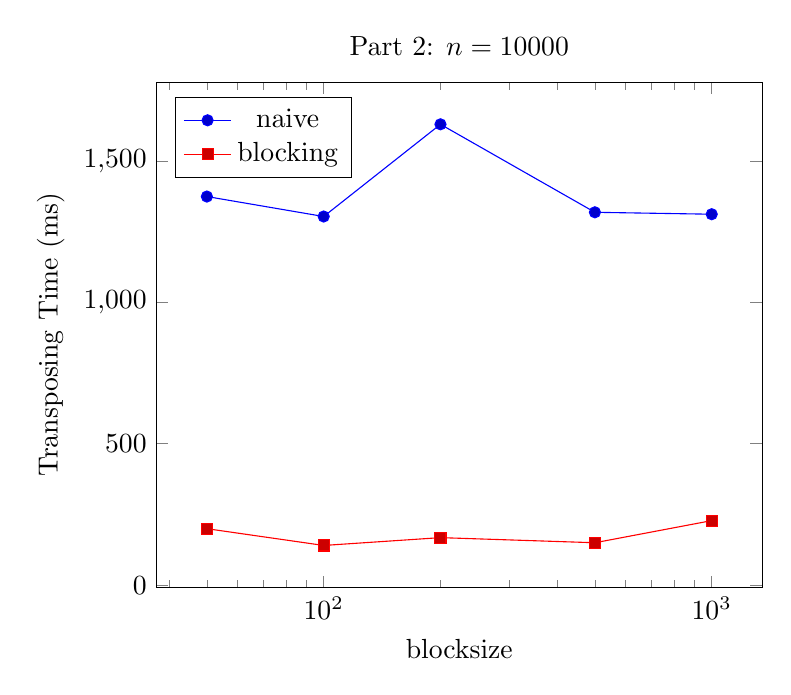
\begin{tikzpicture}
                \begin{semilogxaxis}[legend pos={north west},
                title={Part 2: $n=10000$},
                xlabel={blocksize},
                ylabel={Transposing Time (ms)},
                xmin={},
                ymin={},
                height={8cm},
                ]
                 \addplot+ [] coordinates { (50,1374.33) (100,1303.71) (200,1629.82) (500,1318.62) (1000,1311.8)};
                 \addplot+ [] coordinates { (50,199.625) (100,140.348) (200,168.006) (500,149.924) (1000,228.186)};
                 \legend{naive,blocking,}
                \end{semilogxaxis}
                \end{tikzpicture}                
        \end{figure}
        
        blocksize 增加时性能没有非常明显的变化,会有颠簸现象。因为 Cache 比较大的原因,在一定分块范围内命中率都会比较高,blocksize 并不占据主导因素。比如当 blocksize 为 5000 时,时间立刻上去并逼近普通算法。

        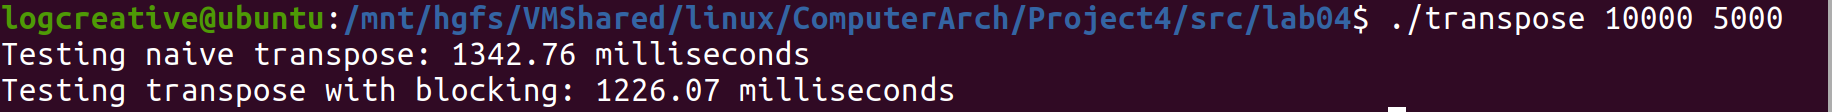
\includegraphics[width=0.8\textwidth]{biggerblock.png}

    \end{steps}
    \clearpage
    \item[4] \textbf{内存山脊}
    
    \begin{itemize}
        \item 运行结果如下:
        
        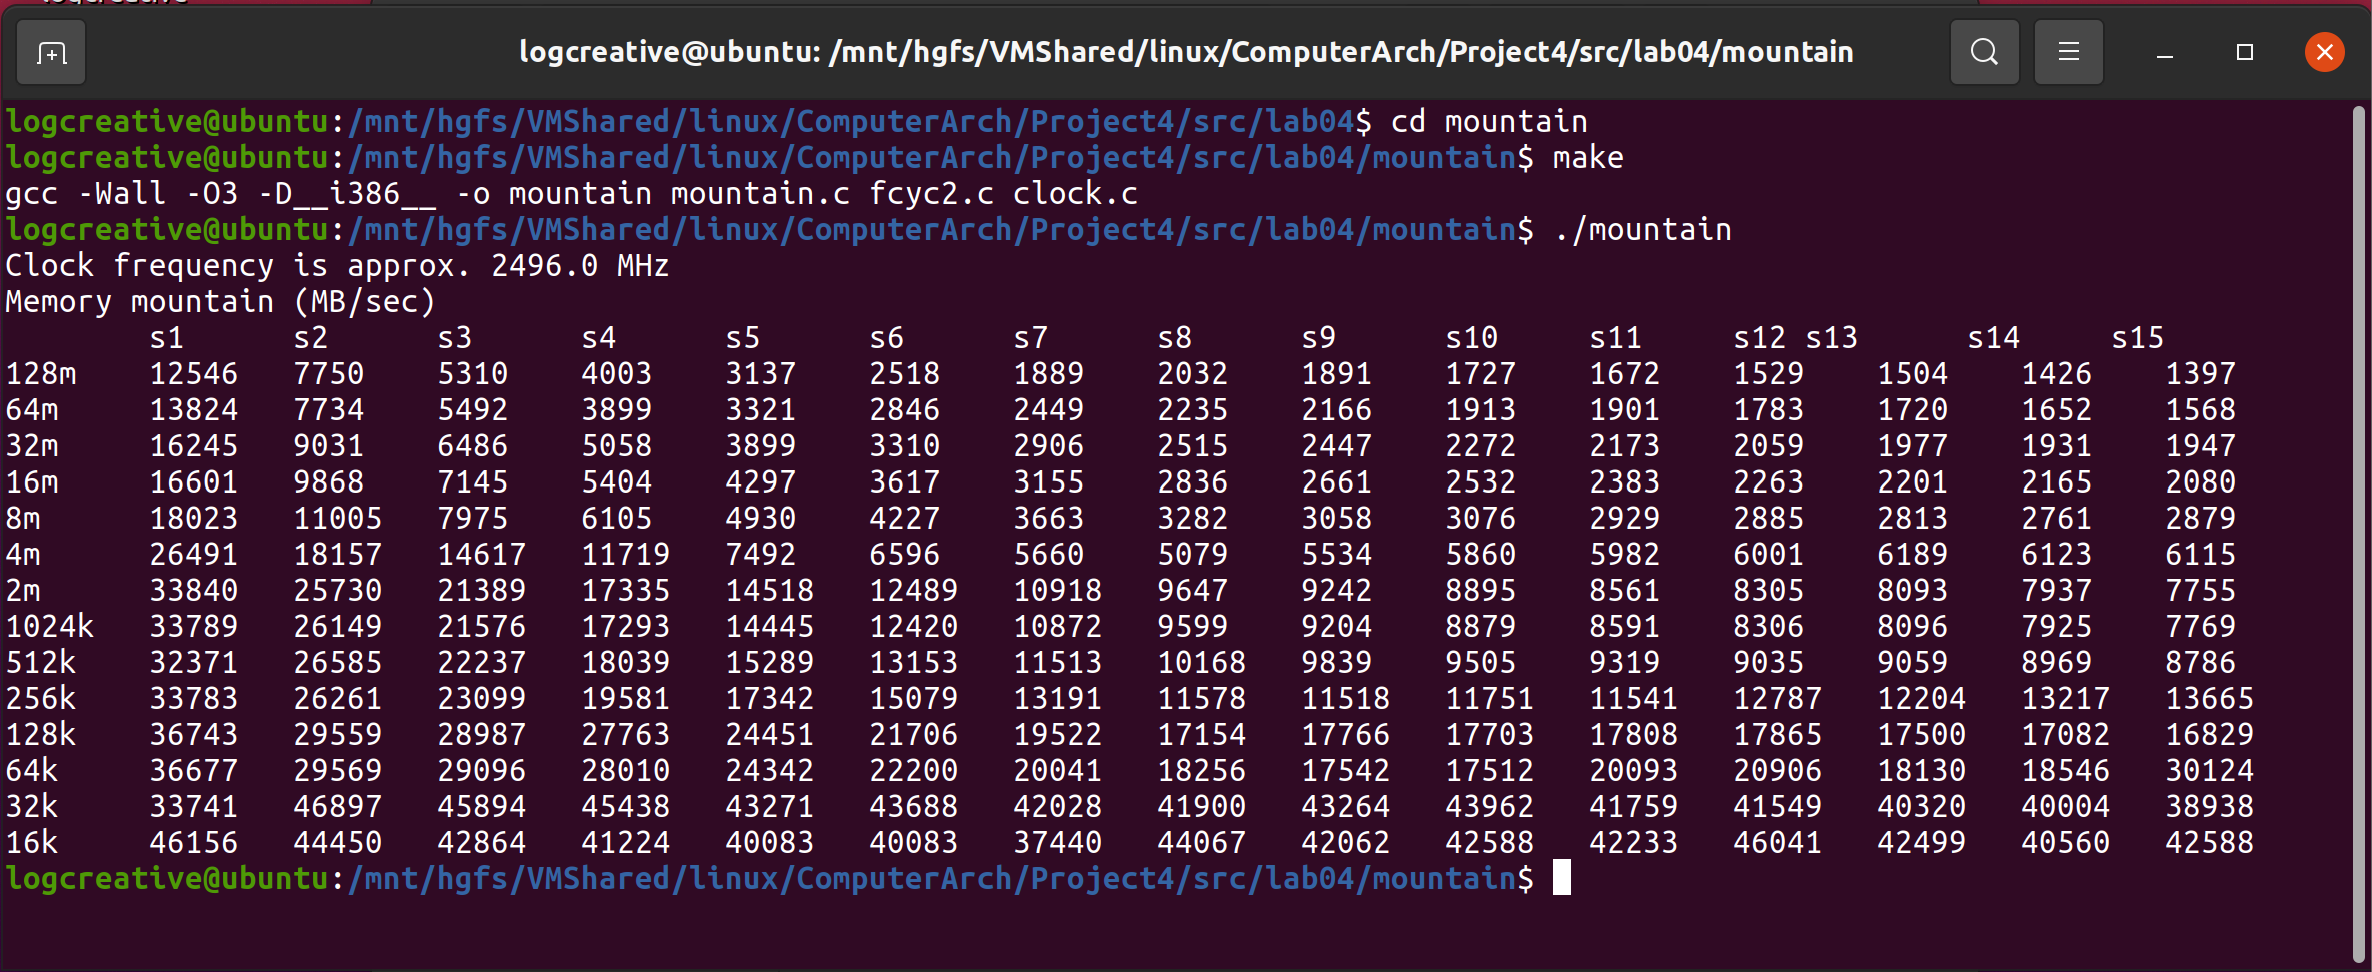
\includegraphics[width=0.8\textwidth]{mountain.png}

        \begin{figure}[h]
            \begin{tikzpicture}
                \begin{axis}[xmin={},
                ymin={0},
                title={stride=8 时间局部性山脊},
                xlabel={工作集大小(bytes)},
                ylabel={读吞吐量(MB$\slash$s)},
                symbolic x coords={16K,32K,64K,128K,256K,512K,1024K,2M,4M,8M,16M,32M,64M,128M},
                ybar,
                enlarge x limits=0.05,
                width=\textwidth,
                height=8cm]
                 \addplot+ [] table[col sep=comma] {perform.csv};
                 \path
                    (axis cs:32K, \pgfkeysvalueof{/pgfplots/ymin})
                    -- coordinate (tmpmin)
                    (axis cs:64K, \pgfkeysvalueof{/pgfplots/ymin})
                    (axis cs:32K, \pgfkeysvalueof{/pgfplots/ymax})
                    -- coordinate (tmpmax)
                    (axis cs:64K, \pgfkeysvalueof{/pgfplots/ymax})
                ;
                \draw[thick, blue] (tmpmin) -- (tmpmax);
                \node [blue,below left of=tmpmax,xshift=0.2cm,yshift=0.5cm] {L1};
                \path
                    (axis cs:256K, \pgfkeysvalueof{/pgfplots/ymin})
                    -- coordinate (tmpmin)
                    (axis cs:512K, \pgfkeysvalueof{/pgfplots/ymin})
                    (axis cs:256K, \pgfkeysvalueof{/pgfplots/ymax})
                    -- coordinate (tmpmax)
                    (axis cs:512K, \pgfkeysvalueof{/pgfplots/ymax})
                ;
                \draw[thick, blue] (tmpmin) -- (tmpmax);
                \node [blue,below left of=tmpmax,xshift=0.2cm,yshift=0.5cm] {L2};
                \path
                    (axis cs:4M, \pgfkeysvalueof{/pgfplots/ymin})
                    -- coordinate (tmpmin)
                    (axis cs:8M, \pgfkeysvalueof{/pgfplots/ymin})
                    (axis cs:4M, \pgfkeysvalueof{/pgfplots/ymax})
                    -- coordinate (tmpmax)
                    (axis cs:8M, \pgfkeysvalueof{/pgfplots/ymax})
                ;
                \draw[thick, blue] (tmpmin) -- (tmpmax);
                \node [blue,below left of=tmpmax,xshift=0.2cm,yshift=0.5cm] {L3};
                \end{axis}
                \matrix [matrix of nodes,xshift=13cm,yshift=5cm] {
                    缓存级别 & 大小 \\
                    L1 & 32K \\
                    L2 & 256K \\
                    L3 & 4M \\
                };
            \end{tikzpicture}
        \end{figure}
        
        % \item 高速缓存配置
        
        % \begin{tabular}{c|c}
        %     缓存级别 & 大小 \\
        %     \hline
        %     L1 & 32K \\
        %     L2 & 128K \\
        %     L3 & 4M \\
        % \end{tabular}

        \item 截图得到 
        
        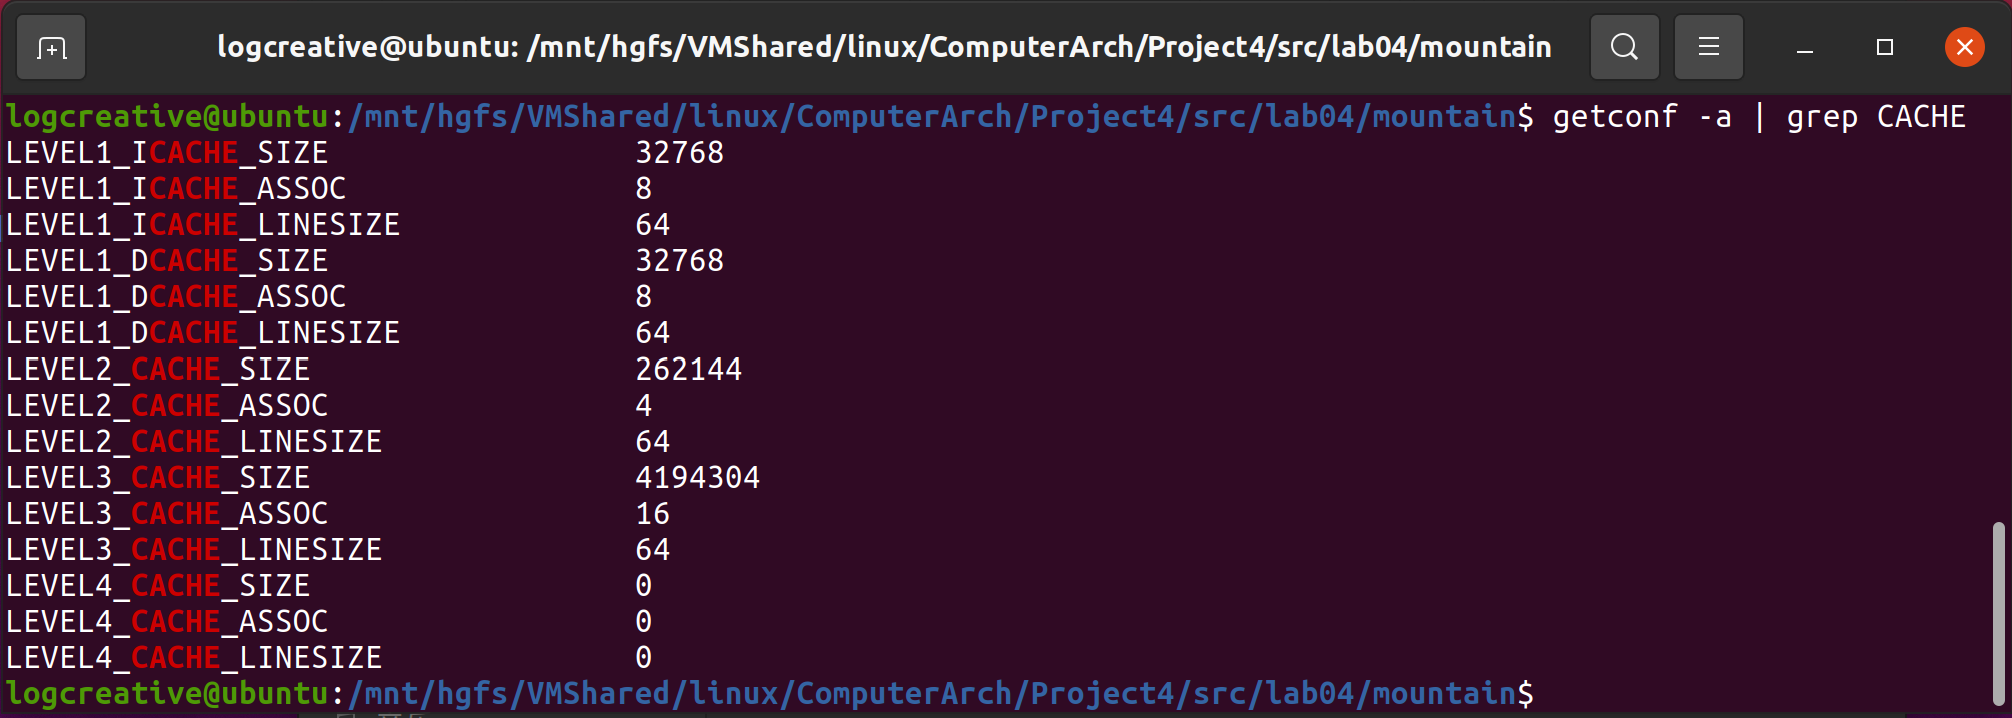
\includegraphics[width=0.8\textwidth]{config.png}

        \begin{tabular}{c|c}
            缓存级别 & 大小(字节) \\
            \hline
            L1 & 32768 \\
            L2 & 262144 \\
            L3 & 4194304 \\
        \end{tabular}

        结果一致。

        \item 固定数组长度为 4MB,有
        
        \begin{figure}[h]
            \begin{tikzpicture}
                \begin{axis}[xmin={},
                ymin={0},
                title={size=4M 空间局部性斜坡},
                xlabel={步长大小($\times$8B)},
                ylabel={读吞吐量(MB$\slash$s)},
                symbolic x coords={s1,s2,s3,s4,s5,s6,s7,s8,s9,s10,s11,s12,s13,s14,s15},
                ybar,
                width=\textwidth,
                height=8cm,
                enlarge x limits=0.05,]
                 \addplot+ [] table[col sep=comma,x=stride,y=throughtput,] {stride.csv};
                 \path
                    (axis cs:s7, \pgfkeysvalueof{/pgfplots/ymin})
                    -- coordinate (tmpmin)
                    (axis cs:s8, \pgfkeysvalueof{/pgfplots/ymin})
                    (axis cs:s7, \pgfkeysvalueof{/pgfplots/ymax})
                    -- coordinate (tmpmax)
                    (axis cs:s8, \pgfkeysvalueof{/pgfplots/ymax})
                ;
                \draw[thick, blue] (tmpmin) -- (tmpmax);
                \end{axis}
                \end{tikzpicture}
        \end{figure}

        图像是一致的。块的大小为 $8\times8=64$ bytes,因为从8开始就是每个高速缓存行一次访问,所以0$\sim$8都是块大小以内的范围。
    \end{itemize}

\end{problems}
\end{document}
